\documentclass[12pt]{article}
\setlength{\oddsidemargin}{0in}
\setlength{\evensidemargin}{0in}
\setlength{\textwidth}{6.5in}
\setlength{\parindent}{0in}
\setlength{\parskip}{\baselineskip}

\usepackage{amsmath,amsfonts,amssymb,bm,graphics,pgfplots,framed,dsfont}
\usepackage[scale=0.75,top=1cm,bottom=3cm]{geometry}

\begin{document}

\textbf{Minh Anh Nguyen }\\
\textbf{Discrete Math\hfill Assignment-7}

\hrulefill

\begin{enumerate}

  \item Refer to Definition 1.10. Show that the divisibility relation | makes the set N of natural numbers a partially ordered set.\\
  \textbf{Reflexivity:}\\
  Because every number $x \in N$ can divides itself. Hence, the divisibility relation is reflexive.\\
  \textbf{Transitivity:}\\
  If $a|b$ and $b|c$ for $a,b,c \in N$. Then $b = a.k$ and $c = b.m$ and $c = a.k.m$. Therefore, c can divides a. Hence, the relation $|$ is transitivity.\\
  \textbf{Antisymmetry:}\\
  If $a|b$ with $a,b \in N$, $a < b$. Hence, a cannot divide a. Therefore, the relation $|$ is antisymmetric.\\
  Hence, the relation $|$ is a partially order set.
  \item Explain why the divisibility relation $|$ does not define a partially ordering on the set Z of integers.\\
  For $x = -1$ and $y = 1$. $x|y$ and also $y|x$. Hence, the relation is not antisymmetric. Therefore, the relation is not a partially ordering set.
  \item Consider the poset $(N,|)$. Are there any minimal elements? Are there any maximal elements? Explain.\\
  Because N = \{1,2,3,4,...$\infty$\}. The minimal element is 1 and there is no maximal elements.
  \item Let A = \{a,b,c,...z\}. In the poset(P(A), $\subset$), find a pair of incomparable elements.\\
  A pair of incomparable elements is (\{a,b,c\},\{d,e,f\}).
  \item Let $W$ be the set of all web pages. For $x, y \in W$, let $x R y$ if you can navigate from $x$ to $y$ by following links (Let's say it always possible to "navigate" from a page to itself; just do nothing.) Explain why R is not a partial ordering.\\
  Let $x,y \in W$, it is possible to navigate from x to y and from y to x. Hence, xRy and yRx. Therefore, R is not antisymmetric and not a partially ordering set.
  \item Let a relation R be defined on the set of real numbers as follows:
  \[xRy \Leftrightarrow 2x + y = 3\]
  Prove that this relation is antisymmetric.\\
  Let: $y = 3 - 2x$\\
  For $yRx$:
  \[yRx \Leftrightarrow 2y + x = 3\]
  \[2(3-2x) + x = 3\]
  \[6-4x + x = 3\]
  \[-3x = -3\]
  \[x = 1\]
  \[y = 3 - 2(1) = 1\]
  Hence, x = y. \\
  Therefore, the relation is antisymmetric.
  \item Explain why the relation R on \{0, 1, 2, 3\} given by
  \[R = \{(0,0),(1,1),(2,2),(3,3),(0,1),(1,2),(2,3),(0,2)\}\]
  is not a partial ordering on \{0, 1, 2, 3\}. Be specific.\\
  Because 1R2 and 2R3 but there is no relation between 1 and 3. Hence, the relation R is not transitive. Therefore, the relation is not a partially ordering set.
  \item Explain why the relation R on \{0, 1, 2, 3\} given by
  \[R = \{(0,0),(1,1),(2,2),(3,3),(0,1),(1,2),(0,2),(2,1)\}\]
  is not a partial ordering on \{0, 1, 2, 3\}. Be specific.\\
  Because 1R2 and 2R1, the relation is not fully antisymmetric. Hence, the relation is not partial ordering.
  \item The Hasse diagram below defines a partial ordering on the set \{0, 1, 2, 3\}. Give the set of ordered pairs corresponding to this relation.
  \begin{center}
    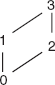
\includegraphics[scale=0.8]{img/img-0.png}
  \end{center}
  \[R = \{(0,1),(1,3),(0,2),(2,3),(0,3),(0,0),(1,1),(2,2),(3,3)\}\]
  \item The Hasse diagram below defines a partial ordering on the set \{0, 1, 2, 3\}. Give the set of ordered pairs corresponding to this relation.
  \begin{center}
    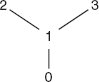
\includegraphics[scale=0.8]{img/img-1.png}
  \end{center}
  \[R = \{(0,1),(0,2),(0,3),(1,2),(1,3),(0,0),(1,1),(2,2),(3,3)\}\]
  \newpage
  \item The divides relation “$|$” defines a partial ordering on the set \{1, 2, 3, 6, 8, 10\}. Draw the Hasse diagram for this poset. What are the maximal elements?
  \begin{center}
    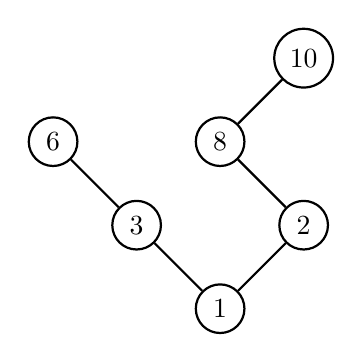
\begin{tikzpicture}[node distance={15mm}, thick, main/.style = {draw, circle}] 
        \node[main] (1) {$1$}; 
        \node[main] (2) [above right of=1] {$2$}; 
        \node[main] (3) [above left of=1] {$3$}; 
        \node[main] (4) [above left of=3] {$6$}; 
        \node[main] (5) [above right of=3] {$8$};
        \node[main] (6) [above right of=5] {$10$}; 
        \draw(1) -- (3);
        \draw(1) -- (2);
        \draw(3) -- (4);
        \draw(2) -- (5);
        \draw(5) -- (6);
        \end{tikzpicture} 
  \end{center}
  The maximal elements are 6 and 10.
  \item Let S = \{1, 2, 3, 5, 10, 15, 20\}. It is a fact that (S, $|$) is a poset. Draw its Hasse diagram.
  \begin{center}
    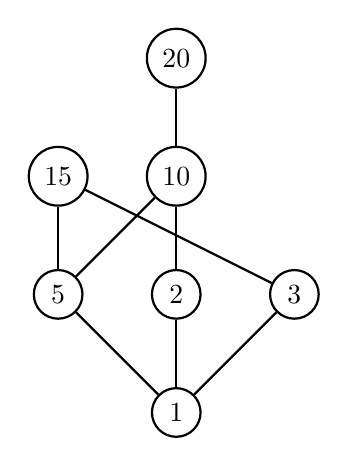
\begin{tikzpicture}[node distance={15mm}, thick, main/.style = {draw, circle}] 
        \node[main] (1) {$1$}; 
        \node[main] (2) [above of=1] {$2$}; 
        \node[main] (3) [right of=2] {$3$}; 
        \node[main] (4) [left of=2] {$5$}; 
        \node[main] (5) [above of=2] {$10$};
        \node[main] (6) [above of=4] {$15$};
        \node[main] (7) [above of=5] {$20$}; 
        \draw(1) -- (3);
        \draw(1) -- (2);
        \draw(2) -- (5);
        \draw(4) -- (5);
        \draw(4) -- (6);
        \draw(4) -- (1);
        \draw(5) -- (7);
        \draw(6) -- (3);
        \end{tikzpicture} 
  \end{center}
  \item Let X be a set of different nonzero monetary values (in U.S. or Canadian cents). In other words, $X \subseteq N$. Define a relation $\vDash$ on x as follows. For $a, b \in X, a \vDash b$ if b can be obtained from a by adding a (possibly empty) collection of dimes (10 cents) and quarters (25 cents). So, for example, $25 \vDash 35$, but $25 \not\vDash 30$. Prove that $\vDash$ is a partial ordering on X.\\
  \textbf{Reflexive: }\\
  For every $a \in X$, $a \vDash a$ because a can add a empty collection of dimes and quarters to become a.\\
  \textbf{Antisymmetric: }\\
  For every $a,b \in X$, if $a \vDash b$ and $a \neq b$, $b$ must be larger than $a$. Hence, $b$ cannot become $a$ by adding a collection of dimes and quarters. Therefore, the relation is antisymmetric.\\
  \textbf{Transitivity: }\\
  For every $a,b,c \in X$, if $a \vDash b$ then $a + 10k + 25z = b$ and if $b \vDash c$ then $b + 10m + 25n = c$. Then $a$ can become $c$ by adding $10k + 25z + 10m + 25n$. Hence, $a \vDash c$. Therefore, the relation is transitive.\\
  Therefore, the relation is partial ordering.
  \newpage
  \item Let X = \{5, 10, 15, 20, 25, 30, 35, 40\}, and let $\vDash$ be as in Problem 13.
  \begin{enumerate}
    \item Draw the Hasse diagram for the poset $(X, \vDash)$.
    \begin{center}
      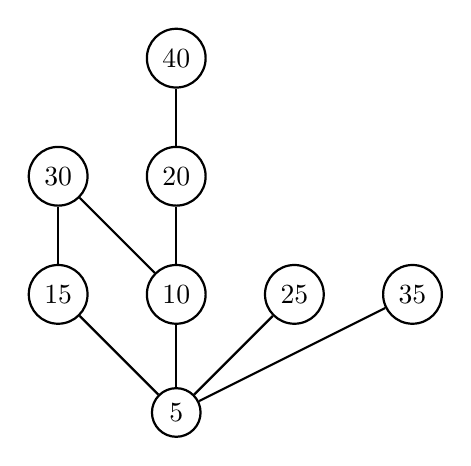
\begin{tikzpicture}[node distance={15mm}, thick, main/.style = {draw, circle}] 
          \node[main] (1) {$5$}; 
          \node[main] (2) [above of=1] {$10$};
          \node[main] (3) [left of=2] {$15$};
          \node[main] (4) [above of=2] {$20$};
          \node[main] (5) [right of=2] {$25$};
          \node[main] (6) [above of=3] {$30$};
          \node[main] (7) [right of=5] {$35$};
          \node[main] (8) [above of=4] {$40$};
          \draw(1) -- (2);
          \draw(1) -- (3);
          \draw(1) -- (5);
          \draw(2) -- (4);
          \draw(3) -- (6);
          \draw(2) -- (6);
          \draw(1) -- (7);
          \draw(4) -- (8);
          \end{tikzpicture} 
    \end{center}
    \item List all the minimal elements of $(X, \vDash)$.\\
    The minimal element of $(X, \vDash)$ is 5.
    \item Give a pair of incomparable elements in $(X, \vDash)$.\\
    A pair of incomparable elements in $(X, \vDash)$ is (20,25).
  \end{enumerate}
  \setcounter{enumi}{18}
  \item Let $X = \{1, 2, 3, 4\}$. Draw the Hasse diagram for the poset $((X), \subset)$.
  \begin{center}
    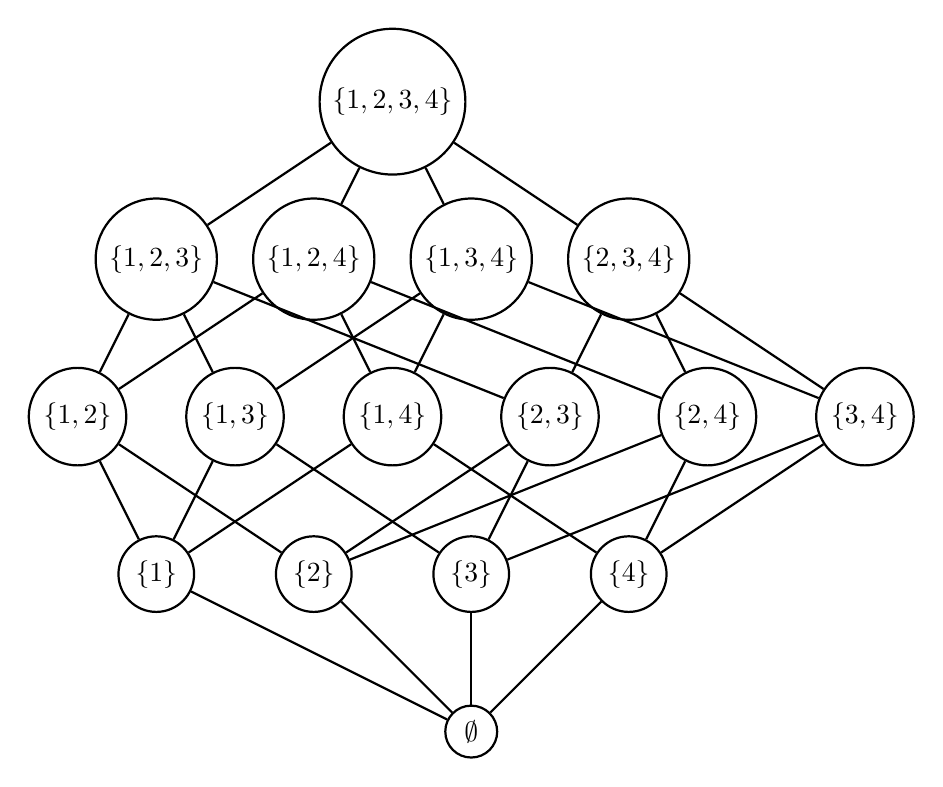
\begin{tikzpicture}[node distance={15mm}, thick, main/.style = {draw, circle}]
        \node[main] (e1) at (0,0) {$\emptyset$};
        \node[main] (e2) at (-4,2) {$\{1\}$};
        \node[main] (e3) at (-2,2) {$\{2\}$};
        \node[main] (e4) at (0,2) {$\{3\}$};
        \node[main] (e5) at (2,2) {$\{4\}$};
        \node[main] (e6) at (-5,4) {$\{1,2\}$};
        \node[main] (e7) at (-3,4) {$\{1,3\}$};
        \node[main] (e8) at (-1,4) {$\{1,4\}$};
        \node[main] (e9) at (1,4) {$\{2,3\}$};
        \node[main] (e10) at (3,4) {$\{2,4\}$};
        \node[main] (e11) at (5,4) {$\{3,4\}$};
        \node[main] (e12) at (-4,6) {$\{1,2,3\}$};
        \node[main] (e13) at (-2,6) {$\{1,2,4\}$};
        \node[main] (e14) at (0,6) {$\{1,3,4\}$};
        \node[main] (e15) at (2,6) {$\{2,3,4\}$};
        \node[main] (e16) at (-1,8) {$\{1,2,3,4\}$};
        
        \draw (e1) -- (e2);
        \draw (e1) -- (e3);
        \draw (e1) -- (e4);
        \draw (e1) -- (e5);
        \draw (e2) -- (e6);
        \draw (e2) -- (e7);
        \draw (e2) -- (e8);
        \draw (e3) -- (e6);
        \draw (e3) -- (e9);
        \draw (e3) -- (e10);
        \draw (e4) -- (e7);
        \draw (e4) -- (e9);
        \draw (e4) -- (e11);
        \draw (e5) -- (e8);
        \draw (e5) -- (e10);
        \draw (e5) -- (e11);
        \draw (e6) -- (e12);
        \draw (e6) -- (e13);
        \draw (e7) -- (e12);
        \draw (e7) -- (e14);
        \draw (e8) -- (e13);
        \draw (e8) -- (e14);
        \draw (e9) -- (e12);
        \draw (e9) -- (e15);
        \draw (e10) -- (e13);
        \draw (e10) -- (e15);
        \draw (e11) -- (e14);
        \draw (e11) -- (e15);
        \draw (e12) -- (e16);
        \draw (e13) -- (e16);
        \draw (e14) -- (e16);
        \draw (e15) -- (e16);
    \end{tikzpicture}
    \end{center}
  \newpage
  \setcounter{enumi}{21}
  \item Let B be the set of all four-digit binary strings; that is,
  \[B = \{0000,0001,0010,0011,...1111\}\]
  Define a relation $\triangleleft$ on B as follows: Let $x, y \in B$, where $x = x_1x_2x_3x_4$ and $y = y_1y_2y_3y_4$. We say that $x \triangleleft y$ if $x_i \leq y_i$ for $i = 1, 2, 3, 4$. In other words, $x \triangleleft y$ if y has a 1 in every position where x does. So, for example, $0101 \triangleleft 0111$ and $0000 \triangleleft 0011$, but $1010 \not\triangleleft 0111$. The relation $\triangleleft$ is called the bitwise $\leq$. Show that $(B, \triangleleft)$ is a poset.
  \textbf{Reflexive: }\\
  For every $a = a_1a_2a_3a_4 \in B$, $a \triangleleft a$ because $a_i \leq a_i$ for $i = 1,2,3,4$. Hence, the relation is reflexive.\\
  \textbf{Antisymmetric: }\\
  For every $a = a_1a_2a_3a_4 \in B$ and $b = b_1b_2b_3b_4 \in B$, if $a \triangleleft b$ and $b \triangleleft a$ then $a = b$ because $a_1a_2a_3a_4 \leq b_1b_2b_3b_4$ and $b_1b_2b_3b_4 \leq a_1a_2a_3a_4$. Hence, the relation is antisymmetric. \\
  \textbf{Transitivity: }\\
  For every $a,b,c \in B$ and $a = a_1a_2a_3a_4, b=b_1b_2b_3b_4, c = c_1c_2c_3c_4$. If $a \triangleleft b$ and $b \triangleleft c$, then $a_i \leq b_i$ and $b_i \leq c_i$ for $i = 1,2,3,4$. Hence, $a_i \leq c_i$ and $a \triangleleft c$. Hence, the relation is transitive.\\
  Therefore, the $(B, \triangleleft)$ is a poset.
  \item Prove that $(B, \triangleleft) \cong (P(\{1,2,3,4\}, \subseteq))$.\\
  We can define a function $f: B \to P(\{1,2,3,4\})$ with that maps each $x = x_1x_2x_3x_4 \in B$ if $x_i = 1$ for $i = 1,2,3,4$ then $i \in f(x)$. Because every elements of B maps exactly to one element of $P(\{1,2,3,4\})$, f is one-to-one correspondence. And because of $\triangleleft$ and $\subseteq$ behave exactly the same for the two sets. Hence, the edges in the Hasse diagram for $(B, \triangleleft)$ correspond exactly to the edges in the Hasse diagram for $(P(\{1,2,3,4\}), \subseteq)$. Therefore, $(B, \triangleleft) \cong (P(\{1,2,3,4\}), \subseteq)$.
  \item In $(B, \triangleleft)$, give a counterexample to show that\\
  \begin{center}
    0000, 0001, 0010, 0011, 0100, 0101, 0110, 0111, 1001, 1000, 1010, 0011, 1100, 1101, 1110, 1111
  \end{center}
  is not a valid topological sort of the elements of B.\\
  Because $0011$ is not the minimal element if $0100$ is not deleted but $0011$ is standing before $0100$, this is not a valid topological sort of the elements of B. 
  \item Perform a topological sort on the elements of B.\\
  A topological sort on the elements of B is:
  \begin{center}
    0000, 0001, 0010, 0100, 1000, 0011, 0101, 0110, 1001, 1010, 1100, 0111, 1110, 1101, 1011, 1111
  \end{center}
  \item Let $F \subseteq N$ be the set of all factors of 210. In the poset $(F, |)$, find the following.
  \begin{enumerate}
    \item $30 \wedge 21$, the meet of 30 and 21.\\
    $30 \wedge 21 = gcd(30,21) = 3$.
    \item $35 \vee 15$, join of 35 and 15.\\
    $35 \vee 15 = lcm(35,15) = 105$.
    \item $2 \wedge 7$.\\
    $2 \wedge 7 = gcd(2,7) = 1$.
    \item $2 \vee 7$.\\
    $2 \vee 7 = lcm(2,7) = 14$.
    \item $\neg 30$, the complement of 30.
    \[\neg 30 = x \text{ with } (30 \wedge x) = 1 \text{ and } (30 \vee x) = 210\]
    \[30 = 2\times3\times5\]
    \[210 = 2\times3\times5\times7\]
    Hence, x = 7 and $\neg 30 = 7$.
  \end{enumerate}

\end{enumerate}
\end{document}